\scanpage{5}

% top edge torn through a letter
$\unsure{P|r}$

N.S.

% slanted
\margin{\deleted{\unsure{par}}}
\diagram{\begin{tikzcd}[ampersand replacement=\&,column sep=2pt,row sep=9pt]
{} \& \text{torsion}\arrow[d,Rightarrow,shift left=4pt,"{\substack{\text{additivité}\\\text{de }\text{\uuline{Pic}}^\tau,\ \text{ou}\\\text{\unsure{raison} spéciale :}\\dA=A}}"] \& {} \& {}\arrow[dd,Rightarrow,"{\substack{\text{\unsure{trivial}}\\\text{par th.}\\\text{des \unsure{int}}}}"'] \& {} \\
{} \& {\equiv}\arrow[u,Rightarrow,shift left=5pt] \& {} \& {} \& {}\\
{} \& \text{équivalence numérique} \& {} \& {} \& {}\arrow[uu,Rightarrow,"{\substack{\text{th. non trivial}\\\text{\unsure{valable} pour les}\\\text{var. non sing}\\\text{projectives}}}"']
\end{tikzcd}}

[critère de Weil. \inserted{\tikz[baseline=(a.base)]\node[draw,rounded corners=7pt,inner sep=2pt](a){\unsure{dû|oui} à Matsusaka};} -]

Il y a une \unsure{dém.} directe plus simple pour les VA (bouquin Lang)

\diagram{\begin{tikzcd}[ampersand replacement=\&,column sep=3pt,row sep=4pt]
|[draw,inner sep=3pt]|{\begin{array}{lc}
\text{algébrique}&\Downarrow\\
\text{torsion}&\Downarrow\\
\equiv&{}\\ \hline
\text{numérique}&{}
\end{array}} \& {\Big\Uparrow\ \Big/\!\Big/} \&
{\displaystyle \leqslant\dim\mathrm{Pic}\,A
\underset{\substack{\text{\deleted{\unsure{théorème}} \inserted{déf.} de Picard ;}\\
\text{égalité ssi}\\\mathrm{Pic}\,A\text{ non}\\\text{singulier}}}{\leqslant}
\dim H^{1}(A,\uline{\unsure{\mathcal O|\mathrm O}}_A)
\underset{\substack{\text{th. de}\\\text{Hopf-Borel}}}{\leqslant}n}
\end{tikzcd}}

\diagram{\begin{tikzcd}[ampersand replacement=\&]
|[draw,rounded corners=16pt,inner sep=5pt]|{\displaystyle
\dim A\overset{\substack{\text{théorie des}\\\text{diviseurs non}\\\text{dégénérés}}}{\leqslant}
\dim\mathrm{Pic}\,A\overset{\text{déf. de Picard}}{\leqslant}
\dim H^1(A,\mathcal O_A)\overset{\text{Hopf-Borel}}{\leqslant}\dim A}
\end{tikzcd}}

\[
A^{**}\quad A\enspace .\quad A^*
\]

\figure{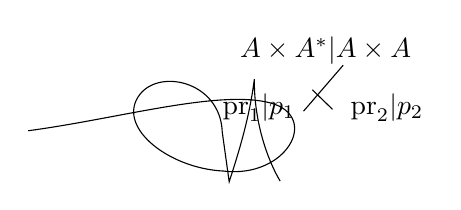
\begin{tikzpicture}[x=.8cm,y=.8cm,line width=.4pt]
\draw (0,.28) .. controls (1.43,.47) and (3.03,.94) .. (3.85,.72) .. controls (4.64,.5) and (4.1,-.48) .. (3.1,-.36) .. controls (2.25,-.32) and (1.43,.31) .. (1.74,.81) .. controls (2.03,1.29) and (3.05,1.08) .. (3.08,.26) -- (3.19,-.53) .. controls (3.39,.08) and (3.52,.56) .. (3.59,1.10) .. controls (3.58,.53) and (3.75,-.10) .. (4.0,-.52);
\node at (4.72,1.55) {$\unsure{A\times A^*|A\times A}$};
\node at (4.68,.65) {$\unsure{\mathrm{pr}_1|p_1}\qquad\unsure{\mathrm{pr}_2|p_2}$};
\draw (4.37,.59) -- (5.00,1.32);
\draw (4.51,.93) -- (4.83,.62);
\end{tikzpicture}}

% archive sheet number: 4

